%\documentclass{clases}
\documentclass[a4paper,12pt, oneside]{book}
\usepackage[skins,minted]{tcolorbox}
\usepackage[utf8]{inputenc}
\usepackage[T1]{fontenc}
\usepackage[spanish, es-tabla]{babel}
\languageshorthands{spanish}
%\usepackage{lmodern} % Usa las fuentes modernas de LaTeX
\usepackage[numbers]{natbib}
%\usepackage{morewrites}
\usepackage{inconsolata}
\usepackage{mdframed}
\usepackage{minted}
\usepackage{bm}
\usepackage{listingsutf8}
\usepackage{subcaption}
\usepackage{amsmath}
\usepackage{amssymb}
\usepackage{graphicx}
\usepackage{hyperref}
\usepackage{longtable}
\usepackage{tabularx}
\usepackage{threeparttable}
\usepackage{array}    % Necesario para centrar horizontal y verticalmente
\usepackage{xcolor}
\usepackage{pdfpages}
%\usepackage{color}
\usepackage{fancyhdr}
\usepackage{menukeys}
\usepackage{appendix}
\usepackage{fontawesome}
\usepackage{comment}
\usepackage{caption}
\usepackage{setspace}
\usepackage[explicit]{titlesec}
\usepackage{booktabs}
\usepackage[a4paper,margin=2cm]{geometry}

%\geometry{top=3cm, bottom=3cm, left=4cm, right=2cm} % Si lo quieres imprimir

\definecolor{green1}{HTML}{1dae28}
\definecolor{green2}{HTML}{afd095}
\definecolor{lightgray}{gray}{0.9}
\definecolor{orange}{RGB}{18,84,183}
\definecolor{titulo}{gray}{0.75}
\definecolor{gray97}{gray}{.97}
\definecolor{gray75}{gray}{.75}
\definecolor{gray45}{gray}{.45}
\definecolor{advertencia}{RGB}{255,178,102}
\definecolor{colorturqueza}{RGB}{178,223,238}
\definecolor{mintedbackground}{rgb}{0.95,0.95,0.95}
\definecolor{lbcolor}{rgb}{0.95,0.95,0.95}
\definecolor{mintedframe}{rgb}{0.0,0.0,0.0}
\definecolor{codebg}{rgb}{0.96,0.96,0.96}
\definecolor{colorurls}{RGB}{107,17,17}
\definecolor{colorsql}{RGB}{255,245,245}
\definecolor{colorreferences}{RGB}{48,134,3}
\definecolor{titulo}{gray}{0.65}			%------ color para fondo del titulo de tablas.

\hypersetup{
	%bookmarks=true,         % show bookmarks bar?
	unicode=true,          % non-Latin characters in Acrobat’s bookmarks
	pdftoolbar=true,        % show Acrobat’s toolbar?
	pdfmenubar=true,        % show Acrobat’s menu?
	pdffitwindow=false,     % window fit to page when opened
	pdfstartview={FitH},    % fits the width of the page to the window
	pdftitle={Reporte final de Robótica},    % title
	%	pdfauthor={},     % author
	pdfsubject={Reporte final de Robótica},   % subject of the document
	%pdfcreator={pdfTeX 3.14159265-2.6-1.40.16 (TeX Live 2016/dev)},   % creator of the document
	%pdfproducer={Panel HJ 2017}, % producer of the document
	pdfkeywords={Manipulador industrial} {Robotica} {ros} {gazebo}, % list of keywords
	%pdfnewwindow=true,      % links in new PDF window
	colorlinks=true,       % false: boxed links; true: colored links
	linkcolor=black,          % color of internal links (change box color with linkbordercolor)
	citecolor=colorreferences,        % color of links to bibliography
	filecolor=magenta,      % color of file links
	urlcolor=blue,           % color of external links
	linkbordercolor={0 0 0}
}

\lstset{
	inputencoding=utf8,
	language=Python,
	frame=Ltb,
	tabsize=2,
	framerule=0pt,
	aboveskip=0.5cm,
	framextopmargin=0pt,
	framexbottommargin=0pt,
	framexleftmargin=0.4cm,
	framesep=0pt,
	rulesep=.0pt,
	backgroundcolor=\color{gray97},
	rulesepcolor=\color{blue},
	%
	stringstyle=\ttfamily,
	showstringspaces = false,
	basicstyle=\small\ttfamily,
	commentstyle=\color{gray45},
	keywordstyle=\bfseries,
	%
	numbers=none,
	numbersep=15pt,
	numberstyle=\tiny,
	numberfirstline = false,
	breaklines=true
}

\setminted[matlab]{%
	breaklines=true,       % activa el ajuste de línea
	breakanywhere=true,    % permite partir en cualquier punto si no hay espacios
	breaksymbolleft=,      % quita el símbolo de continuación
	autogobble            % elimina sangrías comunes
%	fontsize=\footnotesize % reduce tamaño de fuente para que quepa mejor
}

\setminted[bash]{
	bgcolor=mintedbackground,
	fontfamily=tt,
	linenos=true,
	numberblanklines=true,
	numbersep=11pt,
	numbersep=2pt,
	gobble=0,
	frame=leftline,
	framesep=2mm,
	funcnamehighlighting=false,
	tabsize=4,
	obeytabs=false,
	samepage=false,
	showspaces=false,
	showtabs =false,
	texcl=false,
	baselinestretch=1.2,
	fontsize=\footnotesize,
	breaklines=true,
	breaksymbolleft=\ 
}
%\setminted{%
%	breaklines,
%	breaksymbolleft=,      % vacía la marca de continuación
%	breaksymbolright=      % también limpia el símbolo a la derecha
%}


\lstdefinestyle{consola}{
	basicstyle=\footnotesize\bf\ttfamily,
	backgroundcolor=\color{gray75},
}	
\definecolor{gray}{rgb}{0.4,0.4,0.4}
\definecolor{darkblue}{rgb}{0.0,0.0,0.6}
\definecolor{cyan}{rgb}{0.0,0.6,0.6}
\lstset{language=XML}

\lstdefinelanguage{XML}{
	morestring=[b]",
	tabsize=2,
	breaklines=true,
	morestring=[s]{>}{<},
	morecomment=[s]{<?}{?>},
	stringstyle=\color{black},
	identifierstyle=\color{darkblue},
	keywordstyle=\color{cyan},
	numbers=left,
	morekeywords={xmlns,version,type}% list your attributes here
}

\lstdefinestyle{C}{language=C}
\lstdefinestyle{XML}{language=XML}

\DeclareMathOperator{\diag}{diag}

\newtcblisting{terminal}[2][]{
	listing engine=minted,
	listing only,
	#1,
	title=#2,
	minted language=bash,
	colback=mintedbackground,
	top=0mm,
	bottom=0mm
}

\newtcblisting{matlabcode}[2][]{%
  	listing engine=minted,
	listing only,
	title=#2,
	minted language=matlab,
	minted options={%
		linenos,            % activa numeración de líneas
		numbersep=1mm,      % separación texto–números
		breaklines,         % opcional: ajuste automático
		autogobble,          % opcional: recortar sangrías
		frame=leftline,     % línea vertical a la izquierda del bloque
		framesep=1mm,
		tabsize=4,
	},
%	colback=gray!5,
%	colframe=black!70,
	top=0mm,
	bottom=0mm
	#1
}


\newtcblisting{latexcode}[2][]{%
	listing engine=minted,
	listing only,
	title=#2,
	minted language=latex,
	minted options={%
		linenos,            % activa numeración de líneas
		numbersep=1mm,      % separación texto–números
		breaklines,         % opcional: ajuste automático
		autogobble,          % opcional: recortar sangrías
		frame=leftline,     % línea vertical a la izquierda del bloque
		framesep=1mm,
		tabsize=4,
	},
	%	colback=gray!5,
	%	colframe=black!70,
	top=0mm,
	bottom=0mm
	#1
}


\newtcblisting{consolestyle}[2][]{enhanced, listing engine=minted, 
	listing only,#1, title=#2, minted language=bash, 
	coltitle=mintedbackground!35!black, 
	fonttitle=\ttfamily\footnotesize,
	sharp corners, top=0mm, bottom=0mm,
	title code={\path[draw=mintedframe, dashed, fill=mintedbackground](title.south west)--(title.south east);},
	frame code={\path[draw=mintedframe, fill=mintedbackground](frame.south west) rectangle (frame.north east);}
}

\newenvironment{doble}
{\doublespacing
}

%\newcounter{comando}[section]
%\newenvironment{comando}[1][]{\refstepcounter{comando}\par\medskip
	%	\noindent \textbf{Comando~\thecomando. #1} \rmfamily}{\medskip}
%\begin{terminal}{#1}

%\end{terminal}
%}{\medskip}

\graphicspath{{img/}{tablas/}{portada/}}  % Las imágenes se buscarán en la carpeta "img"

\addto\captionsspanish{\renewcommand{\contentsname}{Índice}}

\def\CC{{C\nolinebreak[4]\hspace{-.05em}\raisebox{.4ex}{\tiny\bf ++ \space}}}
\def\Cc{{C\nolinebreak[4]\hspace{-.05em}\raisebox{.4ex}{\tiny\bf ++}}}
\newcommand{\ffolder}[1]{\menu{\faFolderO \space #1}}
\newcommand{\ffile}[1]{\menu{\faFileO \space #1}}
\newcommand{\folder}{\faFolderO \space}
\newcommand{\file}{\faFileO \space}
\newcommand{\world}{\faGlobe \space}
\newcommand{\wworld}[1]{\menu{\faGlobe \space #1}}
\newcommand{\SB}{\{B\}} % Define el sistema del cuerpo
\newcommand{\SI}{\{I\}} % Define el sistema inercial

\newcounter{actividad} % Define un contador llamado "actividad"

\newfloat{Comando}{h}{lot}[chapter]

\renewcommand{\tablename}{Tabla}
\renewcommand{\listtablename}{Índice de tablas}
\renewcommand\listingscaption{Código}
\newcommand{\code}[1]{\colorbox{lightgray}{\texttt{#1}}}

\renewcommand\lstlistingname{Código}
\renewcommand{\appendixname}{Anexo}
\renewcommand{\appendixtocname}{Anexos}
%\renewcommand{\appendixpagename}{Anexo}
\renewcommand\labelitemi{$\bullet$}

\begin{document}
	% Aquí se encuentra el archivo con la portada
	\begin{titlepage}
	\centering
	%-------------------------------------------
	% Logos en una tabla: izquierda, centro y derecha
	\begin{tabular}{@{}p{0.3\textwidth} p{0.3\textwidth} p{0.3\textwidth}@{}}
		
\includegraphics[height=2cm]{tecnm} & 
		\centering 
\includegraphics[height=1.5cm]{SEP} & 
		\raggedleft 
\includegraphics[height=2cm]{ith.jpg} \\
	\end{tabular}
	
	\vspace{2em}
	
	\noindent
	%-------------------------------------------
	%	Información institucional y académica (esquina superior izquierda)
	\begin{minipage}[t]{0.48\textwidth}
		\raggedright
		\small \textbf{%
			Instituto Tecnológico de Hermosillo\\
			Materia: Robótica\\
			Profesor: Medina Gil Lamadrid, Jesús Iván%
		}
	\end{minipage}%
	\hfill
	%	fecha actual (esquina superior derecha), en letras pequeñas y en negrita.
	\begin{minipage}[t]{0.48\textwidth}
		\raggedleft
		\small \textbf{\today}
	\end{minipage}
	
	\vspace{2em}
	
	%-----------------------------------------
	% Unidad y Título de la tarea en letras grandes y en negrita
	{\large \textbf{Unidad 1: Morfología del robot}}\\
	{\Huge \textbf{Tipos de Sensores
}}
		
	\vspace{1em}
	
	%---------------------------------------
	% Tabla con la información del equipo
	%---------------------------------------
	% Encabezado del equipo
	\begin{center}
		{\Large \textbf{Equipo 2}}
	\end{center}
	
	\vspace{1em}
	
	% Tabla de integrantes:
	% Cada fila contiene: foto (columna izquierda) y datos del integrante (columna derecha)
	\begin{center}
		\begin{tabular}{c c}
			\begin{tabular}{c}
				
\includegraphics[height=3cm]{perfil1.jpg} \\
				\textbf{Encinas Clark},\\ Efrain Adrian \\ \texttt{l21330568@hermosillo.tecnm.mx} \\ 
			\end{tabular} &
			\begin{tabular}{c}
				
\includegraphics[height=3cm]{perfil2.jpg} \\
				\textbf{Arredondo Solano,}\\ Yairee Daniela \\ \texttt{21330531@hermosillo.tecnm.mx} \\ 
			\end{tabular} \\ \vspace{2em}
			\begin{tabular}{c}
				
\includegraphics[height=3cm]{perfil3.jpg} \\
				\textbf{Vasquez Romero,}\\ Diego Jesus \\ \texttt{21330708@hermosillo.tecnm.mx} \\ 
			\end{tabular} &
			\begin{tabular}{c}
				
\includegraphics[height=3cm]{perfil4.jpg} \\
				\textbf{Cancio Elizondo ,}\\ Valeria Alejandra \\ \texttt{21330545@hermosillo.tecnm.mx} \\
			\end{tabular}
		\end{tabular}
	\end{center}

\end{titlepage}

	\onehalfspacing
	\frontmatter
	\pagestyle{plain}  % numeración en páginas preliminares
	\titleformat{\chapter}
	{\bfseries\huge}
	{}
	{0pt}
	{~\raisebox{-1.5pt}{}
	\\\filleft #1 \\\vspace{.25cm}\titlerule[1.5pt]}
	
	% ---------------------------------------
	% índices
%	\clearpage   % o \cleardoublepage, según prefieras
	\newpage
	\phantomsection    % crea un nuevo destino para hyperref
	\addcontentsline{toc}{chapter}{Índice general}
	\tableofcontents
	
%	\clearpage
	\newpage
	\phantomsection
	\addcontentsline{toc}{chapter}{Índice de figuras}
	\listoffigures
	
	\hypersetup{
		linkcolor=red
	}
	
	% ---------------------------------------
	% Estilo de encabezado y pie de página
	\mainmatter
	\pagestyle{fancy}
	\fancyhead{}
	\fancyhead[L]{\leftmark}
	\fancyhead[R]{}
	\fancyfoot[L]{\parbox[l]{\textwidth-1cm}{\rightmark}}
	\fancyfoot[C]{}
	\fancyfoot[R]{\thepage}
	\renewcommand{\footrulewidth}{0.5pt}
	%\fancyfoot[RO,LE]{Diseño de modelo para simulación 3D de VANT tipo cuadricóptero}
	
	\titleformat{\chapter}
	{\bfseries\huge}
	{}
	{0pt}
	{\titlerule[3pt]~\raisebox{-1.5pt}{\sc{\chaptername}~\thechapter}~\titlerule[3pt]%
		\\\vspace{.05cm}\titlerule\\\filcenter #1 \\\vspace{.25cm}\titlerule}
	
	% Capítulo 1: Introducción
	\chapter{Desarrollo} \label{chap:desarrollo}
En este capítulo hablarán sobre el proyecto del robot que hicieron y los pasos para llevarlo a cabo, así como algunas funciones de Matlab. Que lo hicieron con Solidworks y lo convirtieron a URDF para usarlo con ROS.
	
	% Capítulo 2: Marco Teórico
	\chapter{Desarrollo} \label{chap:desarrollo}
En este capítulo hablarán sobre el proyecto del robot que hicieron y los pasos para llevarlo a cabo, así como algunas funciones de Matlab. Que lo hicieron con Solidworks y lo convirtieron a URDF para usarlo con ROS.
	
		\section{Cinemática} \label{sec:cinematica}

La cinemática es una rama de la física que estudia el movimiento de los objetos sólidos en función del tiempo, sin considerar las causas (fuerzas) que lo originan. Este análisis se basa en variables como la posición, la velocidad y la aceleración, y considera tres elementos fundamentales: el espacio, el tiempo y el móvil. En el contexto de la robótica, se aplica especialmente a sistemas de cuerpos rígidos como los manipuladores, describiendo sus trayectorias sin involucrar dinámicas.

En robótica, la cinemática se clasifica principalmente en dos tipos: \textbf{cinemática directa} y \textbf{cinemática inversa}. La primera permite determinar la posición y orientación del efector final a partir de los valores articulares del robot, mientras que la segunda se enfoca en calcular los valores articulares que permiten alcanzar una posición y orientación deseadas del efector final.

\subsection{Cinemática Directa}

La cinemática directa (o directa geométrica) establece la relación entre los ángulos articulares del robot y la posición y orientación del efector final. Para esta tarea, comúnmente se emplea el método de Denavit-Hartenberg (DH), que permite representar de forma sistemática la configuración espacial del robot mediante transformaciones homogéneas.

Dichas transformaciones permiten obtener no solo la ubicación del efector final, sino también su orientación en el espacio. Además, conceptos como el jacobiano geométrico son fundamentales para analizar la velocidad y aceleración del sistema en función de sus variables articulares.

Un desarrollo detallado del análisis computacional aplicado a este modelo puede encontrarse en la \hyperref[sec:proceso_cinematica]{sección del proceso de Cinemática}.

\subsection{Cinemática Diferencial}

s
Dentro de la robótica la cinemática diferencial se enfoca en el estudio de cómo cambian las velocidades del robot conforme se van moviendo sus articulaciones. Se relacionan las velocidades articulares con las velocidades lineales y angulares del efector final. Nos permite calcular cómo se mueve y controlar la velocidad del efector final. 
El Jacobiano es una matriz la cual relaciona directamente estas dos velocidades. Está traduce velocidades del espacio articular al espacio cartesiano. El Jacobiano de un robot con n articulaciones tiene las siguientes características:
  \\
-6 filas \\
-n número de columnas.\\

\begin{figure}[h]
	\centering
	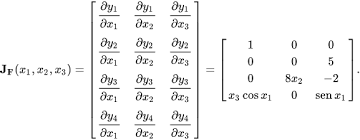
\includegraphics[width=0.5\linewidth]{img/jacobiano}
	\caption{Matriz de Jacobiano}
	\label{fig:jacobiano}
\end{figure}
		
		\section{ROS} \label{sec:ros}
Aquí se explicará un poco sobre qué es ROS.
\begin{figure}[h]
	\centering
	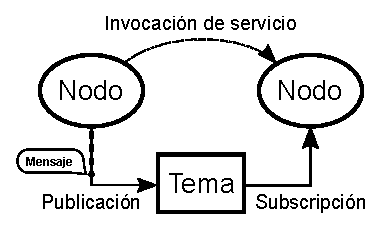
\includegraphics[width=0.5\linewidth]{img/ROS_concepts}
	\caption{Diagrama de comunicación de ROS}
	\label{fig:rosconcepts}
\end{figure}

También están interesantes las animaciones que vienen en la \href{https://docs.ros.org/en/humble/Tutorials/Beginner-CLI-Tools/Understanding-ROS2-Topics/Understanding-ROS2-Topics.html}{página de ROS} \cite{ros2-understanding-topics}, pero lamentablemente no se pueden poner animaciones en el reporte.

\subsection{Nodo (Node)}
\subsection{Tema (Topic)}
\subsection{Mensaje (Message)}
\subsection{Servicio (Service)}
\subsection{Gazebo}
\subsection{RViz}

		
		\section{Dinámica} \label{sec:dinamica}

La dinámica estudia las fuerzas y torques y su efecto en el movimiento del robot. Forma general de la ecuación dinámica es: 
 
\begin{figure}[h]
	\centering
	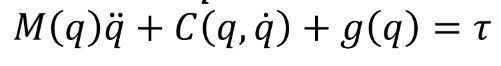
\includegraphics[width=0.5\linewidth]{img/ECDINA}
	\caption{Ecuación dinámica}
	\label{fig:ECDINA}
\end{figure} 
 \newpage
  donde:
  q: Coordenadas articulares generalizadas\\[5pt]
  M(q): Matriz de masa o inercia\\[5pt]
  C(q,q’):Fuerzas centrífugas y de Coriolis\\[5pt]
  g(q): Fuerzas de gravedad\\[5pt]
  torque = Fuerzas (o pares) generalizadas\\[5pt]
  

\subsection{Matriz de masa o inercia}


La matriz de masa M(q) representa cómo la masa del robot está distribuida y cómo esa masa influye en la resistencia al movimiento. Es una matriz simétrica y positiva definida la cual depende de la configuración q del robot y está formada por los parámetros físicos del sistema, como: \\[5pt]
-Las masas de los eslabones \\[5pt]
-Longitudes de los brazos \\[5pt]
-Momentos de inercia de cada segmento. \\[5pt]

Esta matriz se obtiene a partir del modelo dinámico del robot usando el método de Euler-Lagrange y no solo describe la resistencia al movimiento sino también define el límite superior de la aceleración que puede alcanzar un robot bajo una cantidad de fuerza o torque. Esto nos indica que a mayor inercia menor será la aceleración máxima que puede lograrse con un mismo torque. 

\subsection{Matriz de coriolis}

La matriz de Coriolis representa los efectos que causan las fuerzas centrífugas y fuerzas de Coriolis las cuales surgen cuando el robot se encuentra en movimiento. Estas fuerzas aparecen debido a las velocidades articulares y depende de la posición y velocidad. 
Se basa en derivadas parciales de la matriz de inercia y se utilizan los coeficientes de Christoffel. 

\subsection{Vector de gravedad}

El vector de gravedad representa las fuerzas que ejercen el peso en los eslabones dependiendo de su configuración. Cuando el robot está extendido horizontalmente, el torque necesario para mantener su propio peso es el máximo ya que se necesita más torque para sostener el peso de los eslabones que están más alejados del eje del motor. 

\subsection{Fricción}

La fricción es la fuerza que se opone al movimiento entre dos superficies que se encuentran en contacto.

\subsubsection{Fricción estática o seca}

Es la fuerza la cual impide el movimiento de un objeto en contacto con otro objeto o superficie. La velocidad debe ser igual a 0.
 
\subsubsection{Fricción dinámica o viscosa}

Es la fuerza que se opone al movimiento cuando el objeto  ya está en  movimiento. La velocidad es diferente a cero. 



\subsection{Perturbaciones}
Una perturbación es cualquier fenómeno que causa un cambio o alteración en el comportamiento de un sistema. 

		
		\section{Control}
Si quieren, pueden comentar esta parte, pero si quieren, expliquen el diagrama de bloques de la \autoref{fig:diagrama-de-robot-industrial}.

\begin{figure}[h]
	\centering
	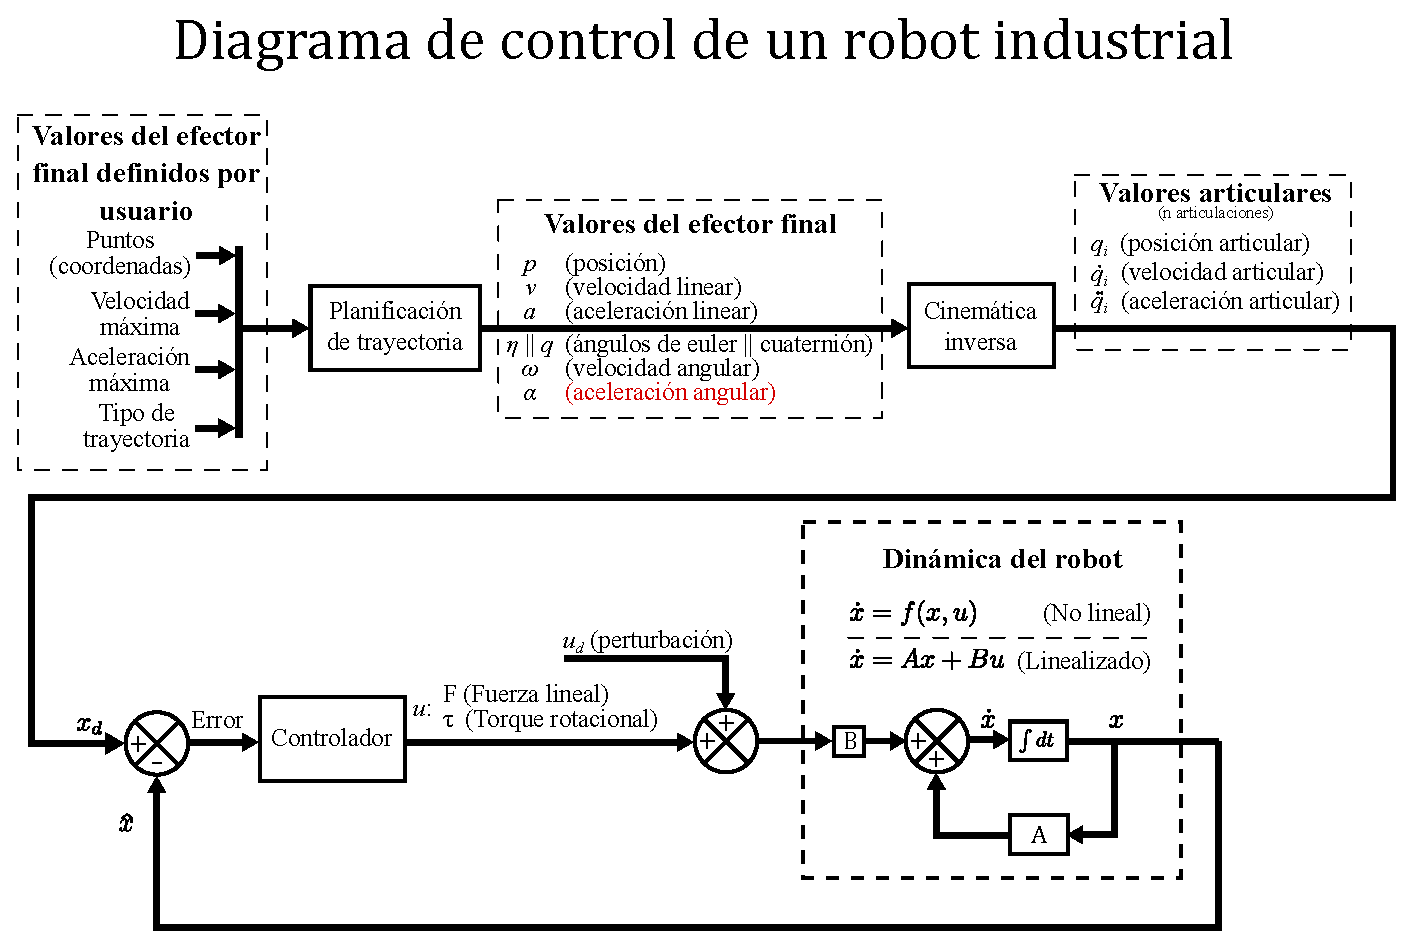
\includegraphics[width=\linewidth]{img/Diagrama_robot_industrial}
	\caption{Diagrama de bloques de un robot industrial}
	\label{fig:diagrama-de-robot-industrial}
\end{figure}

	
	% Capítulo 3: Desarrollo
	\chapter{Desarrollo} \label{chap:desarrollo}
En este capítulo hablarán sobre el proyecto del robot que hicieron y los pasos para llevarlo a cabo, así como algunas funciones de Matlab. Que lo hicieron con Solidworks y lo convirtieron a URDF para usarlo con ROS.
	
		\section{Características del Robot} \label{sec:caracteristicas_del_robot}

\begin{table}[H]
	\centering
	\begin{tabular}{|c|c|c|c|c|c|c|c|c|c|}
		\hline
		N & $\theta$ (rad) & $d$ & $a$ & $\alpha$ (rad) & Tipo & Min (rad) & Max (rad) & $\dot{q}_{\text{max}}$ (rad/s) & $\ddot{q}_{\text{max}}$ (rad/s$^2$) \\
		\hline
		1 & 0.00  & 52   & 0    & -1.57 & r & -3.14 & 3.14 & 3.14 & 6.28 \\
		2 & -1.57 & 0    & 50   & 0.00  & r & -1.57 & 1.31 & 3.14 & 6.28 \\
		3 & 0.00  & 0    & 14.5 & -1.57 & r & -1.57 & 1.05 & 3.14 & 6.28 \\
		4 & 0.00  & 47.5 & 0    & 0.00  & r & -3.14 & 3.14 & 3.14 & 6.28 \\
		\hline
	\end{tabular}
	\caption{Parámetros DH y límites articulares del robot por articulación (valores en radianes)}
	\label{tab:parametros_dh_articulaciones}
\end{table}

\bigskip
\noindent
\textbf{Donde:}
\begin{description}
	\item[N] Número de la articulación.
	\item[\(\theta\)] Ángulo articular en radianes.
	\item[\(d\)] Desplazamiento articular (cm).
	\item[\(a\)] Longitud del eslabón (cm).
	\item[\(\alpha\)] Ángulo de torsión DH en radianes.
	\item[tipo] ‘r’ para articulación rotacional, ‘p’ para prismática.
	\item[\(q_{\min}\), \(q_{\max}\)] Límites de posición en radianes.
	\item[\(\dot q_{\max}\)] Límite de velocidad en radianes/s.
	\item[\(\ddot q_{\max}\)] Límite de aceleración en radianes/s².

\end{description}


		
			\subsubsection{Motores} \label{subsubsec:motores}

El sistema de accionamiento del robot incorpora distintos tipos de motores, seleccionados estratégicamente según los requerimientos específicos de torque, precisión y control de cada componente:

\begin{itemize}
	\item \textbf{Motores servo SureServo2 (modelo SV2M-220B):} Se utilizaron dos motores \textit{brushless} de corriente alterna, cada uno con una potencia nominal de 2 kW y un par de sujeción de 84.5 lb-in. Están equipados con encoders de alta resolución de 24 bits (16,777,216 pulsos por revolución) y freno integrado. Estos motores operan con entrada trifásica y ofrecen velocidades de hasta 3000 rpm, siendo ideales para tareas que requieren alta precisión y control dinámico. Fueron acoplados a cajas reductoras de precisión para optimizar su desempeño mecánico.
	
	\item \textbf{Motor de corriente continua Weonefit (DC 24 V, 45 W):} Este motor de engranajes proporciona una salida de 220 rpm con un par nominal de 30 Nm, siendo adecuado para aplicaciones de bajo consumo energético que requieren buen torque a velocidades moderadas. Su construcción en materiales metálicos y plásticos lo hace robusto para tareas de baja complejidad mecánica.
	
	\item \textbf{Motor paso a paso STEPPERONLINE con caja reductora planetaria 47:1:} Este conjunto incorpora un motor NEMA 23 bipolar con un torque de sujeción de hasta 40 Nm y una corriente nominal de 2.8 A por fase. Gracias a la caja planetaria, se obtiene una alta relación de reducción, lo que permite movimientos controlados, precisos y con alto torque, útiles para tareas que no demandan retroalimentación continua.
\end{itemize}


\subsubsection{Eslabones} \label{subsubsec:eslabones}

La estructura mecánica del robot está compuesta por eslabones metálicos que forman los brazos y segmentos articulados. Cada eslabón fue diseñado considerando tanto la distribución de masas como la longitud efectiva de trabajo, asegurando estabilidad dinámica y resistencia estructural. A continuación se describen sus características principales:

\begin{itemize}

	\item \textbf{Eslabón 1:} Masa de 17.68 kg, longitud de 0.28 m.
	\item \textbf{Eslabón 2:} Masa de 15.5 kg, longitud de 0.30 m.
	\item \textbf{Eslabón 3:} Masa de 6.5 kg, longitud de 0.25 m.
	\item \textbf{Eslabón 4:} Masa de 6.5 kg, longitud de 0.35 m.
\end{itemize}

Estas dimensiones fueron seleccionadas considerando el equilibrio entre la carga que deben soportar, la eficiencia en la transmisión del movimiento y la minimización del momento de inercia en cada articulación. Además, su disposición permite al robot alcanzar posiciones complejas y ejecutar trayectorias con precisión y estabilidad.

			
			\subsection{Límites y propiedades dinámicas de las articulaciones} \label{subsec:limites_propiedades}

Básicamente, explicarán lo que aparece en la \autoref{tab:parametros_robot}: Parámetros de Denavit Hartenberg y límites del robot, específicamente lo que aparece después de \code{tipo}. Como no completamos la tarea de dinámica,. pueden comentar esta subsección del documento principal.
		
		\section{Proceso de Cinemática} \label{sec:proceso_cinematica}

\subsection{Cinemática Directa}

La cinemática directa permite determinar la posición y orientación del efector final del robot a partir de los valores articulares. A continuación, se explican las secciones más relevantes del código empleado.

\subsubsection*{Creación de la estructura del robot}

Se leyó la tabla DH del robot desde un archivo CSV, y se construyó su modelo mediante la función \texttt{crear\_robot}, que genera las matrices de transformación homogénea necesarias para cada eslabón.

\begin{matlabcode}{matlab}
	dh = readtable('datos\tabla_DH\robotnuestro.csv');
	robot = crear_robot(dh, A0);
\end{matlabcode}

\subsubsection*{Generación de trayectorias articulares}

Para simular el movimiento del robot, se generaron trayectorias para las posiciones (\texttt{q}), velocidades (\texttt{dq}) y aceleraciones (\texttt{ddq}) articulares. Estas se utilizaron como entrada para los cálculos de cinemática.

\begin{matlabcode}{matlab}
	[q, dq, ddq] = trayectoria_q(robot, t, periodo);
\end{matlabcode}

\subsubsection*{Cálculo de posición y orientación del efector}

Se recorrió cada instante de tiempo para actualizar la configuración del robot, obteniendo así la posición y orientación del efector final en el espacio. La orientación se calculó en ángulos de Euler a partir de la matriz de rotación.

\begin{matlabcode}{matlab}
	for k = 1:length(t)
	robot = actualizar_robot(robot, q(:,k));
	posicion(:,k) = robot.T(1:3,4,end);
	R(:,:,k) = robot.T(1:3,1:3,end);
	orientacion(:,k) = rotMat2euler(R(:, :, k), secuencia);
	end
\end{matlabcode}

\subsubsection*{Cálculo de velocidades y aceleraciones}

Usando el Jacobiano geométrico, se calcularon la velocidad y aceleración lineal y angular del efector final. Se aplicó la fórmula:

\[
\dot{x} = J(q)\,\dot{q}, \quad \ddot{x} = J(q)\,\ddot{q} + \dot{J}(q)\,\dot{q}
\]

\begin{matlabcode}{matlab}
	vel_linear(:,k)  = Jv(:,:,k) * dq(:,k); 
	vel_angular(:,k) = Jw(:,:,k) * dq(:,k);  
	
	acel_linear(:,k)  = Jv(:,:,k) * ddq(:,k) + dJv(:,:,k) * dq(:,k); 
	acel_angular(:,k) = Jw(:,:,k) * ddq(:,k) + dJw(:,:,k) * dq(:,k);
\end{matlabcode}

\subsubsection*{Visualización}

Se generó una animación para validar visualmente el movimiento del robot. Esta animación fue útil para corroborar que la cinemática directa estaba funcionando correctamente.

\begin{matlabcode}{matlab}
	g = crear_grafica_robot();
	for k = 1:length(t_animacion)
	robot = actualizar_robot(robot, q_anim(:,k));
	g = dibujar_robot(g, robot);
	end
\end{matlabcode}

Las gráficas de resultados correspondientes a posición, orientación, velocidad y aceleración se presentan en la sección de \autoref{chap:resultados}.

\subsection{Cinemática Diferencial}

La cinemática diferencial permite calcular la velocidad y aceleración del efector final a partir de las velocidades y aceleraciones articulares, usando el Jacobiano del robot. A continuación, se presenta la implementación en MATLAB dividida en pasos relevantes.

\subsubsection*{Actualización de la configuración del robot}

Para cada instante de tiempo, se actualizó el modelo del robot con los valores articulares correspondientes.

\begin{matlabcode}{matlab}
	for k = 1:length(t)
	robot = actualizar_robot(robot, q(:,k));
\end{matlabcode}

\subsubsection*{Extracción de posición y orientación}

Se extrajo la posición y la matriz de rotación del efector final, y luego se convirtieron en ángulos de Euler para analizar la orientación.

\begin{matlabcode}{matlab}
	posicion(:,k)   = robot.T(1:3,4,end);
	R(:,:,k)        = robot.T(1:3,1:3,end);
	orientacion(:,k)= rotMat2euler(R(:,:,k), secuencia);
\end{matlabcode}

\subsubsection*{Cálculo del Jacobiano geométrico}

Se obtuvo el Jacobiano geométrico, que relaciona las velocidades articulares con las velocidades del efector final.

\begin{matlabcode}{matlab}
	[Jv(:,:,k), Jw(:,:,k)] = jac_geometrico(robot);
\end{matlabcode}

\subsubsection*{Cálculo de velocidades del efector final}

A partir del Jacobiano y de las velocidades articulares se obtuvieron la velocidad lineal y angular del efector final.

\begin{matlabcode}{matlab}
	vel_linear(:,k)  = Jv(:,:,k) * dq(:,k);
	vel_angular(:,k) = Jw(:,:,k) * dq(:,k);
\end{matlabcode}

\subsubsection*{Derivada del Jacobiano (diferencias finitas)}

Para calcular las aceleraciones se necesitó la derivada del Jacobiano, la cual se obtuvo mediante diferencias finitas.

\begin{matlabcode}{matlab}
	if k > 1
	dJv(:,:,k) = (Jv(:,:,k) - Jv(:,:,k-1)) / dt;
	dJw(:,:,k) = (Jw(:,:,k) - Jw(:,:,k-1)) / dt;
	end
\end{matlabcode}

\subsubsection*{Cálculo de aceleraciones del efector final}

Finalmente, se calcularon las aceleraciones lineales y angulares del efector usando la fórmula completa de la cinemática diferencial:

\[
\dot{x} = J(q)\,\dot{q}, \quad \ddot{x} = J(q)\,\ddot{q} + \dot{J}(q)\,\dot{q}
\]

\begin{matlabcode}{matlab}
	acel_linear(:,k)  = Jv(:,:,k) * ddq(:,k) + dJv(:,:,k) * dq(:,k);
	acel_angular(:,k) = Jw(:,:,k) * ddq(:,k) + dJw(:,:,k) * dq(:,k);
	end
\end{matlabcode}

\subsubsection*{Resultados}

Los datos obtenidos fueron utilizados para generar gráficas de velocidad y aceleración tanto lineal como angular, así como para validar el comportamiento dinámico del efector final durante la trayectoria.



\subsection{Cinemática Inversa}

La cinemática inversa permite encontrar los valores articulares que lleva al efector final a una posición deseada en el espacio. A continuación, se describen las secciones más relevantes del código empleado.

\subsubsection*{Definición de la posición y orientación inicial}

Se definieron los valores iniciales de posición y orientación del efector final, así como la matriz de transformación homogénea inicial.

\begin{matlabcode}{matlab}
	x = 0; y = 0; z = 0;
	p_robot = [x; y; z];
	phi = 0; theta = 0; psi = 0;
	ori_robot = deg2rad([phi; theta; psi]);
	R_inicial = euler2rotMat(ori_robot, "XYZ");
	A0 = [R_inicial p_robot; zeros(1,3) 1];
\end{matlabcode}

\subsubsection*{Creación del modelo del robot}

Se leyó la tabla DH desde un archivo y se construyó el modelo del robot.

\begin{matlabcode}{matlab}
	dh = readtable('datos\tabla_DH\robotnuestro.csv');
	robot = crear_robot(dh, A0);
\end{matlabcode}


\subsubsection*{Resolución de la cinemática inversa}

Se empleó un método iterativo basado en descenso del gradiente para minimizar el error entre la posición deseada y la alcanzada. En caso de quedar atrapado en un mínimo local, se evaluaron múltiples candidatos articulares.

\begin{matlabcode}{matlab}
	tol = 1e-6;
	max_iter = 100;
	alpha = 1.0;
	numSamples = 9;
	
	for i = 1:n
	[q_sol(:,i), p_sol(:,i)] = cinematica_inv(robot, pos_puntos(:,i), ...
	tol, max_iter, alpha, numSamples);
	end
\end{matlabcode}

\subsubsection*{Generación de trayectoria articular continua}

Se interpolaron las posiciones articulares resultantes de la cinemática inversa para obtener perfiles suaves de velocidad y aceleración mediante trayectorias trapezoidales.

\begin{matlabcode}{matlab}
	delta_q = abs(q_sol(:,2) - q_sol(:,1));
	t_final = max(2 * delta_q ./ robot.dqMax);
	numSamples = 201;
	
	[q, dq, ddq, t, pp] = trapveltraj(q_sol, numSamples, ...
	'Acceleration', robot.ddqMax, ...
	'EndTime', 5);
\end{matlabcode}

\subsubsection*{Validación mediante cinemática directa}

Se aplicó cinemática directa a las trayectorias articulares interpoladas para verificar que la posición alcanzada correspondiera con la deseada.

\begin{matlabcode}{matlab}
	[posicion, vel_linear, acel_linear, orientacion, ...
	vel_angular, acel_angular] = cinematica_dir(robot, q, dq, ddq, t, "XYZ");
\end{matlabcode}

\subsubsection*{Animación}

Se generó una animación del robot en movimiento usando la configuración articular evaluada en cada instante de tiempo.

\begin{matlabcode}{matlab}
	g = crear_grafica_robot();
	for k = 1:length(t_animacion)
	for i = 1:robot.NGDL
	q_anim(i) = ppval(cell2mat(pp(i)), t_animacion(k));
	end
	robot = actualizar_robot_completo(robot, q_anim);
	g = dibujar_robot(g, robot);
	end
\end{matlabcode}


		
		\section{Control}
Si quieren, pueden comentar esta parte, pero si quieren, expliquen el diagrama de bloques de la \autoref{fig:diagrama-de-robot-industrial}.

\begin{figure}[h]
	\centering
	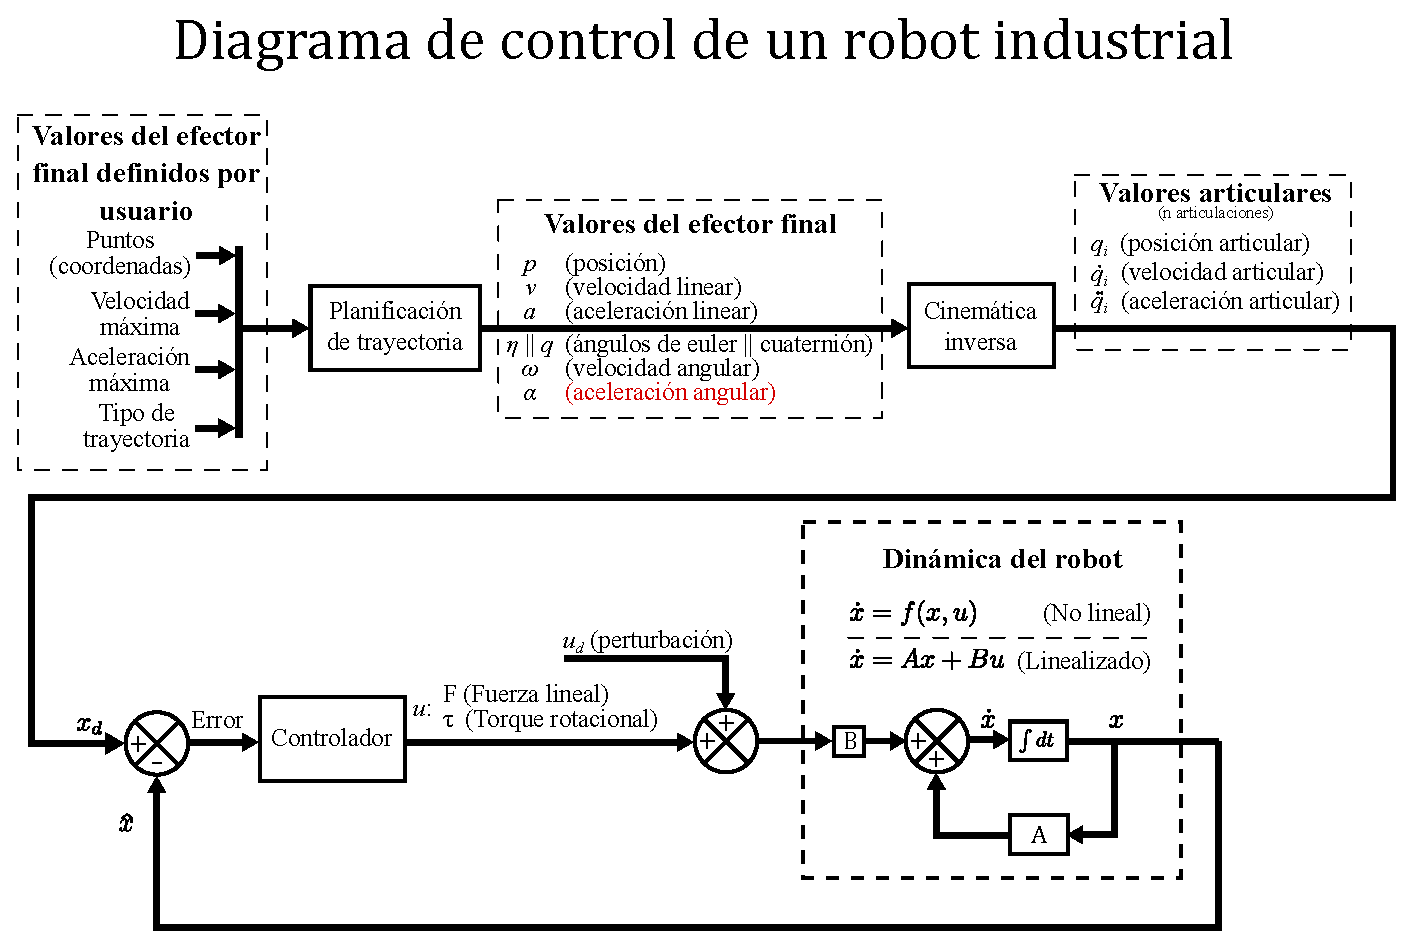
\includegraphics[width=\linewidth]{img/Diagrama_robot_industrial}
	\caption{Diagrama de bloques de un robot industrial}
	\label{fig:diagrama-de-robot-industrial}
\end{figure}

		
		\input{capitulos/Desarrollo/Simulación}
	
	% Capítulo 4: Resultados
	

\chapter{Resultados} \label{chap:resultados}

\begin{figure}[H]  % <-- Este cambio es clave para que no se brinque
	\centering
	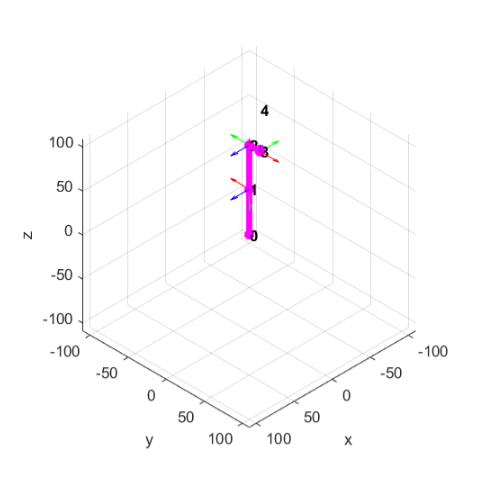
\includegraphics[width=0.7\linewidth]{img/grafica1directa}
	\caption{Representación tridimensional del robot con su sistema de coordenadas en cada eslabón. Se observa la posición y orientación del efector final en el espacio.}
	\label{fig:grafica1directa}
\end{figure}
La Figura 4.1 muestra la representación tridimensional del robot luego de aplicar la cinemática directa. Se visualizan los cuatro eslabones, así como los sistemas de coordenadas asociados a cada uno. Esta figura permite verificar visualmente que la configuración espacial del robot corresponde con los valores articulares definidos en la simulación.



\begin{figure}[H]
	\centering
	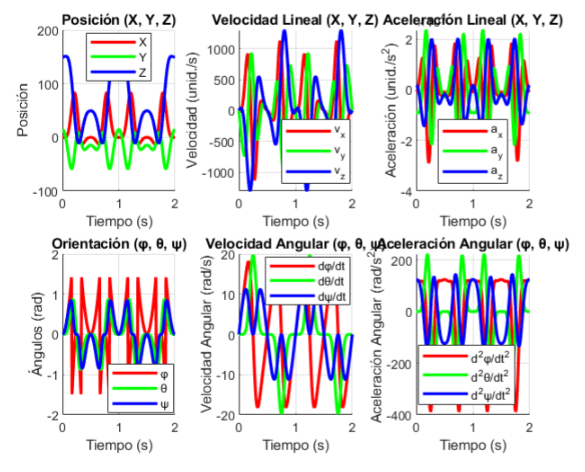
\includegraphics[width=0.9\linewidth]{img/imagen2directa}
	\caption{Resultados de la cinemática directa: posición, velocidad y aceleración lineal (superior), orientación, velocidad y aceleración angular (inferior) del efector final en función del tiempo.}
	\label{fig:imagen2directa}
\end{figure}
La Figura 4.2 presenta los resultados obtenidos a partir de la cinemática directa. En la primera fila se observan las componentes X, Y y Z de la posición, velocidad y aceleración lineal del efector final. En la segunda fila, se grafican los ángulos de Euler, así como sus derivadas primera y segunda (velocidad y aceleración angular). Estas gráficas permiten analizar el comportamiento dinámico del efector final a lo largo del tiempo.



\begin{figure}[H]
	\centering
	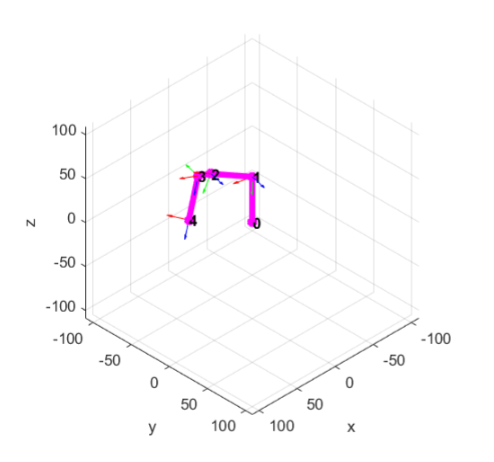
\includegraphics[width=0.7\linewidth]{img/inversa1}
	\caption{Representación 3D del robot en su entorno espacial durante la ejecución de la trayectoria.}
	\label{fig:inversa1}
\end{figure}
La Figura 4.3 muestra la animación del robot siguiendo una trayectoria predefinida en el espacio tridimensional. Las líneas representan los eslabones del robot, mientras que los ejes indican la orientación de cada articulación. Esta visualización fue generada durante la simulación de la cinemática inversa, donde el robot ajusta sus juntas para alcanzar puntos objetivos definidos por la trayectoria cartesiana.


\begin{figure} [H]
	\centering
	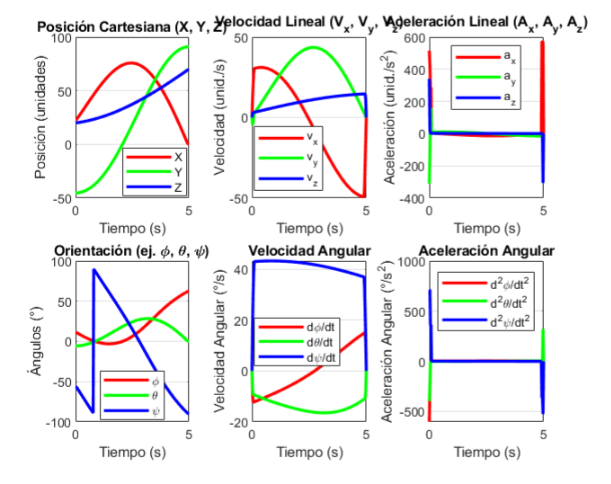
\includegraphics[width=0.9\linewidth]{img/inversa2}
	\caption{Comportamiento de la trayectoria cartesiana del efector final: posición, velocidad y aceleración lineal y angular.}
	\label{fig:inversa2}
\end{figure}
La Figura 4.4 muestra la evolución temporal de la posición (X, Y, Z), la velocidad y aceleración lineal del efector final, así como su orientación (ángulos de Euler), velocidad angular y aceleración angular. Estos resultados provienen de la cinemática directa aplicada a los ángulos articulares obtenidos mediante la cinemática inversa. Se puede observar que las curvas siguen un perfil suave, lo cual es crucial para garantizar un movimiento continuo y estable del robot.



\begin{figure} [H]
	\centering
	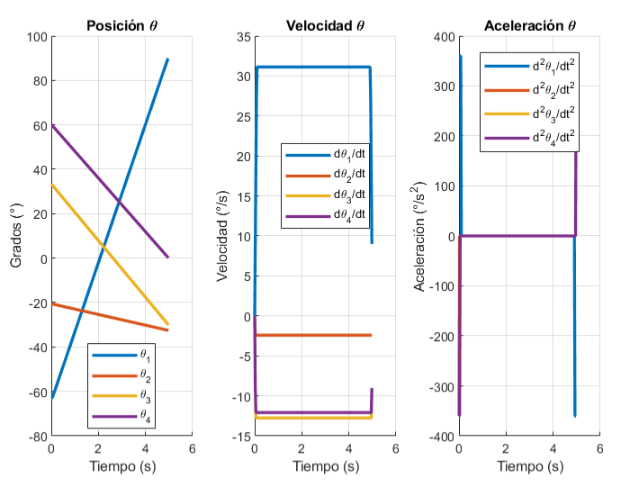
\includegraphics[width=0.9\linewidth]{img/inversa3}
	\caption{Trayectoria articular del robot: posición, velocidad y aceleración de las juntas.}
	\label{fig:inversa3}
\end{figure}
La Figura 4.5 representa el comportamiento de las variables articulares del robot a lo largo del tiempo. Se observa cómo cada articulación cambia su posición en grados, así como su velocidad y aceleración angular. Las trayectorias fueron generadas utilizando perfiles trapezoidales, lo que permite una transición suave entre los estados iniciales y finales, respetando los límites de velocidad y aceleración definidos para el robot.


\newpage

A continuación se muestran diversas imagenes del video de la simulación completa, donde se muestran diferentes poses como estado cero, straight up, pick object, lift object, opposite y place object. 


\begin{figure} [H]
	\centering
	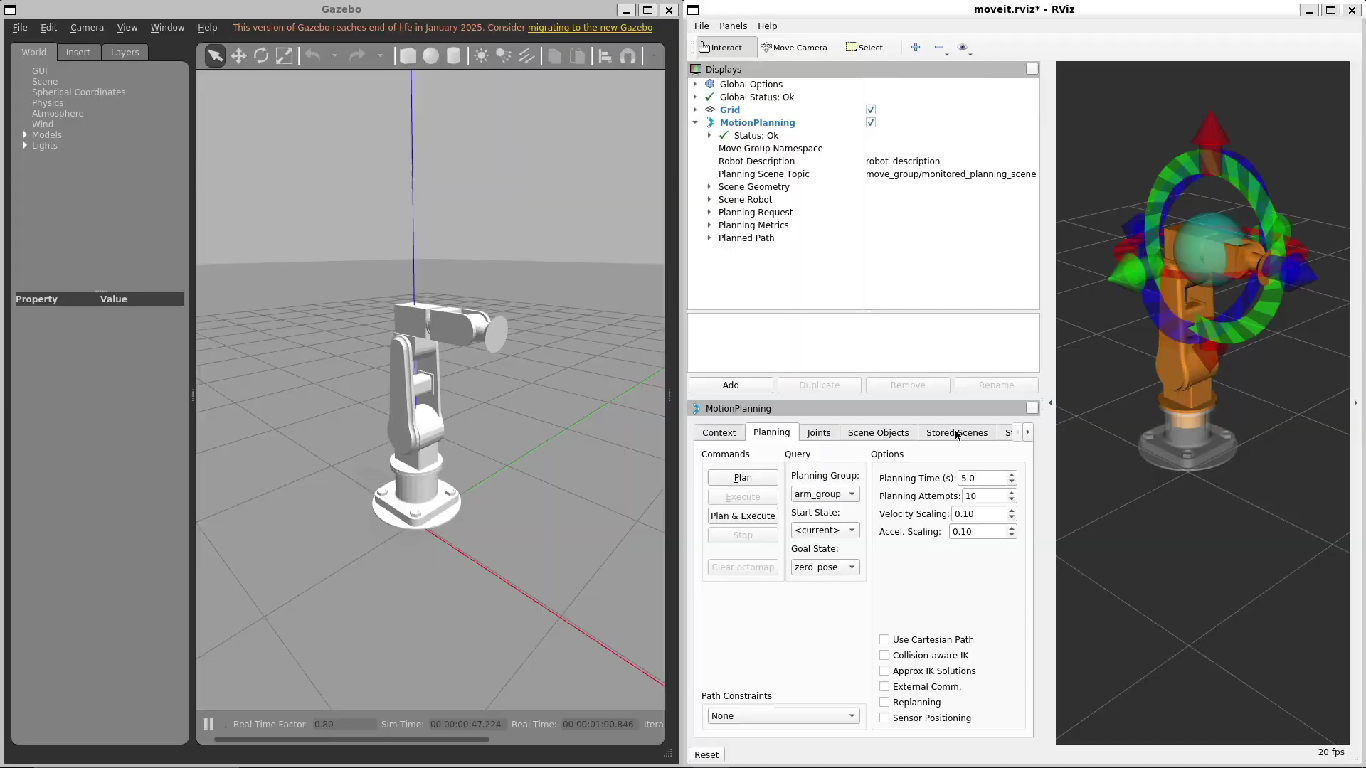
\includegraphics[width=0.9\linewidth]{img/SIMU1}
	\caption{Simulación de robot en estado cero.}
	\label{fig:SIMU1}
\end{figure}


\begin{figure} [H]
	\centering
	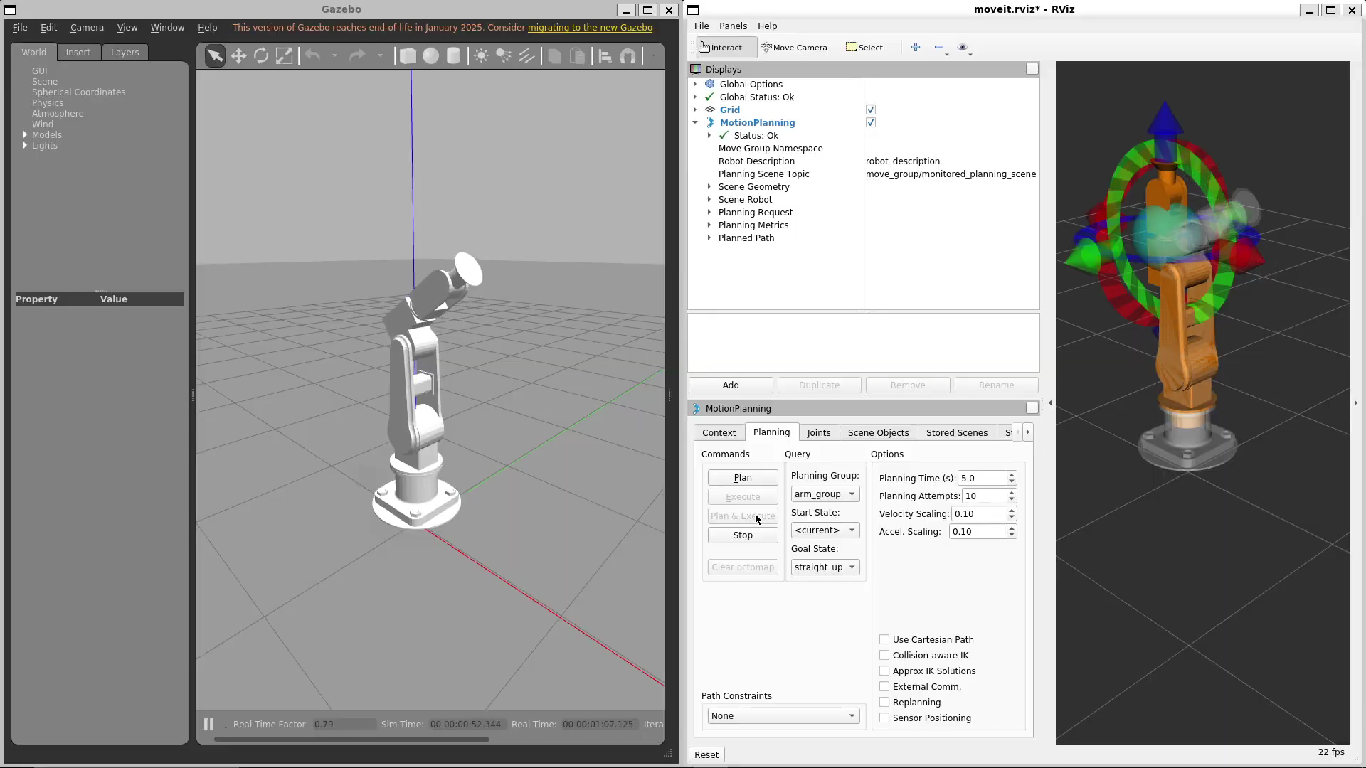
\includegraphics[width=0.9\linewidth]{img/SIMU2}
	\caption{Simulación de robot en trayectoria a straight up.}
	\label{fig:SIMU2}
\end{figure}


\begin{figure} [H]
	\centering
	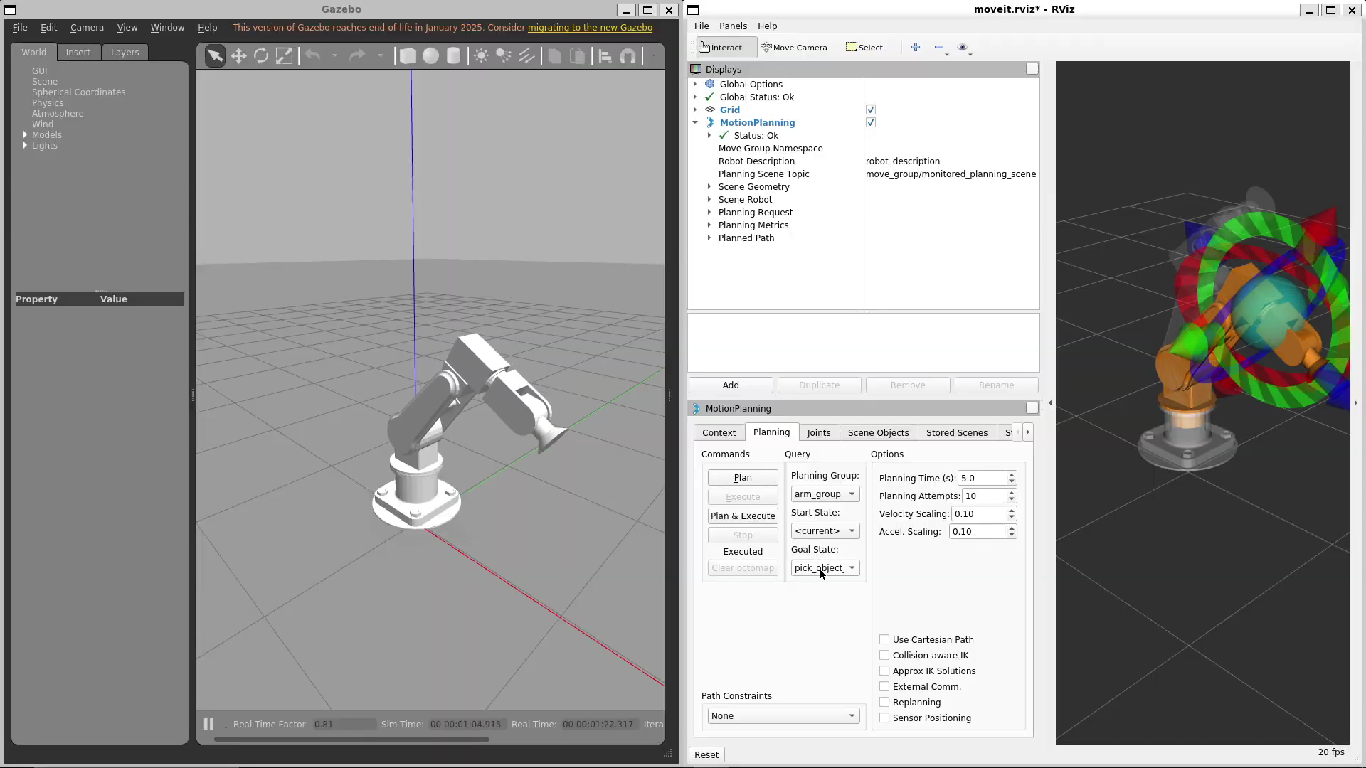
\includegraphics[width=0.9\linewidth]{img/SIMU6}
	\caption{Simulación de robot en trayectoria a pick object.}
	\label{fig:SIMU6}
\end{figure}


\begin{figure} [H]
	\centering
	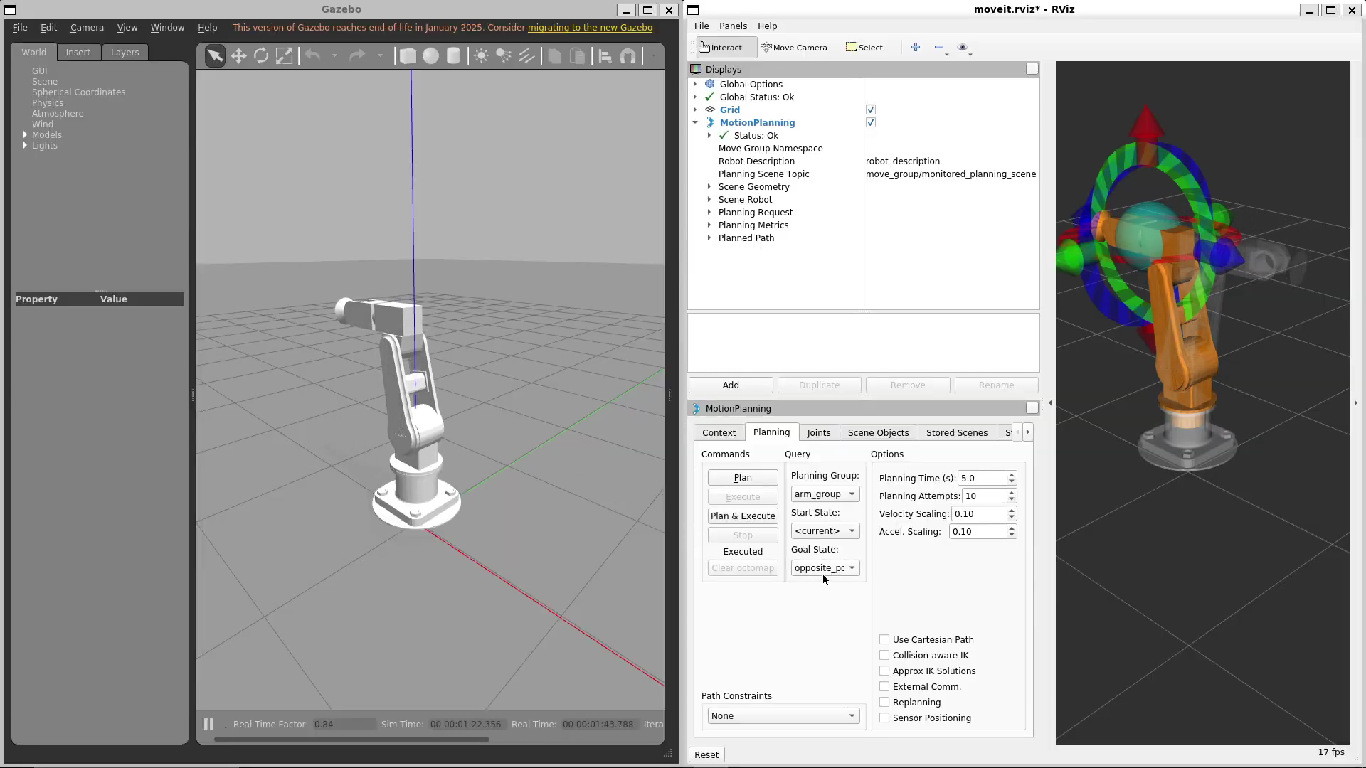
\includegraphics[width=0.9\linewidth]{img/SIMU9}
	\caption{Simulación de robot en opposite}
	\label{fig:SIMU9}
\end{figure}

\begin{figure} [H]
	\centering
	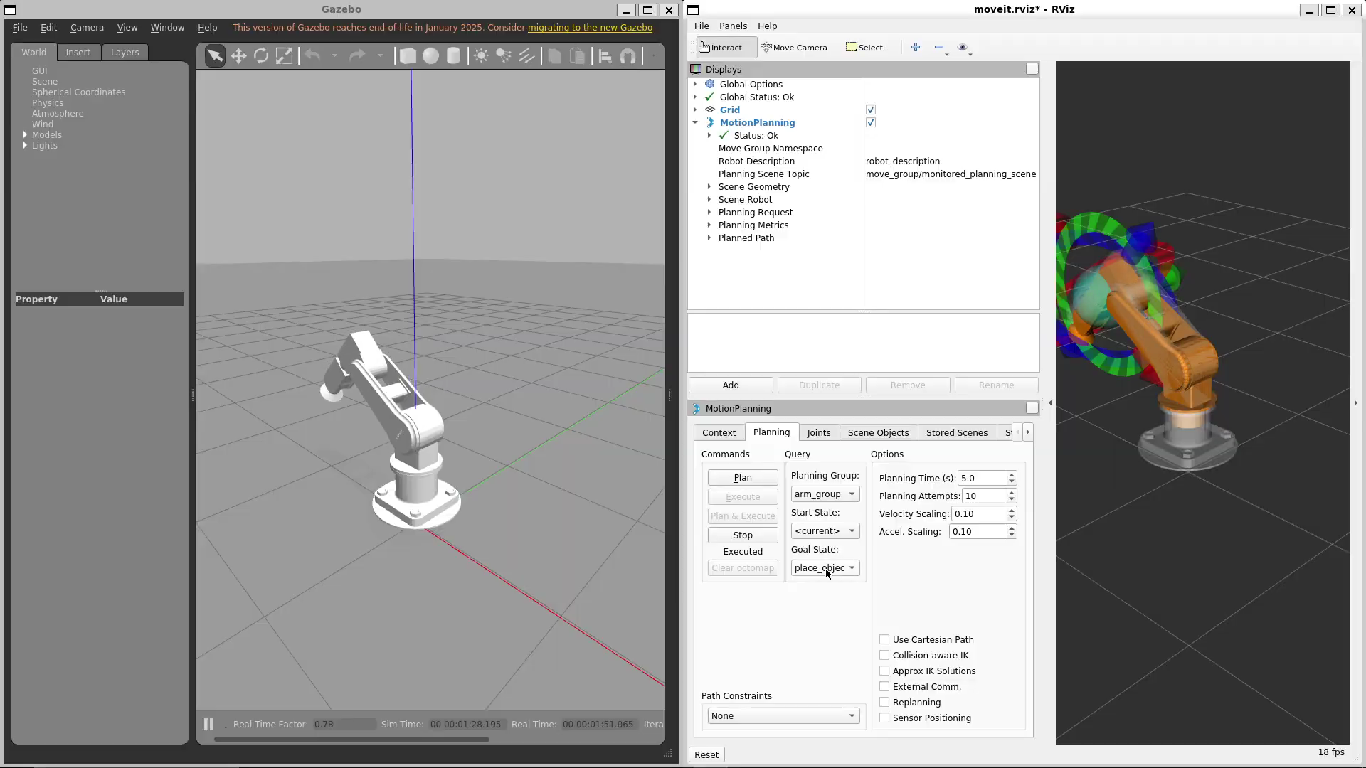
\includegraphics[width=0.9\linewidth]{img/SIMU11}
	\caption{Simulación de robot en place object.}
	\label{fig:SIMU11}
\end{figure}







	
	% Capítulo 5: Conclusiones
	\chapter{Conclusiones} \label{sec:conclusiones}
	\section{Valeria Cancio}
Conclusiones y comentarios de Juancito, explicando los problemas que tuvo y lo que aprendió.
	\section{Panchito}
Conclusiones y comentarios de Panchito, explicando los problemas que tuvo y lo que aprendió.
	\section{Lupita}
Conclusiones y comentarios de Lupita, explicando los problemas que tuvo y lo que aprendió.
	\section{Diego Vásquez}
Personalmente, me divertí mucho en esta materia. Al comienzo me sentí un poco perdido, pues la verdad no comprendía del todo el por qué de lo que veíamos en clase, fue hasta que nos adentramos más en la parte práctica del robot que mis dudas fueron disipadas y por fin comprendí el propósito de la teoría. Entrando más en detalle, mi parte favorita fue todo lo de ROS. Las principales dificultades de la realización de nuestro robot, sobre todo la parte simulada, fue la poca familiaridad que se tenía con el entorno, así como lo “viejo” del tutorial, pues hubieron algunas partes que tuvimos que resolver por nuestra cuenta.

En general, fue muy entretenido simular, experimentar e incluso batallar con las irregularidades que nos iban apareciendo. Pienso que es una muy buena materia para familiarizarse un poco con la realidad de la industria, y, asimismo, aprender un poco mientras se conoce más sobre el mundo de la robótica y sus aplicaciones.
		
	\titleformat{\chapter}
	{\bfseries\huge}
	{}
	{0pt}
	{~\raisebox{-1.5pt}{}
		\\\vspace{.05cm}\titlerule\\\filcenter #1 \\\vspace{.25cm}\titlerule}
	%{\titlerule\\\vspace{.25cm}\filcenter #1 \\\vspace{.25cm}\titlerule}
	\bibliographystyle{IEEEtranN}
	\newpage\label{bibliografia}
	\addcontentsline{toc}{chapter}{Bibliografía}
	
	% Pulsa Ctrl + Clic Izquierdo en bibliografia para entrar.
	\bibliography{bibliografia}
\end{document}


